\chapter{Background}\label{chap:background}

As detailed in Section \ref{sec:problem}, the failure detection problem can be viewed as a sequence classification problem.

The first step is to develop methods to classify the samples instead of the entire sequences.
In order to do so, multiple machine learning methods are possible such as decision trees and neural networks.

In the next few sections we will discuss how these approaches were used in literature and the results that they obtained.
Moreover, for the five methods we actually implemented we will discuss the theory behind them and the motivation to use them.

\section{Decision Tree}\label{sec:decisiontree}

A decision tree represents a flowchart in the form of if-else statements.
Because of this, one of its main advantages is the fact that it is fairly easy to interpret it and to understand how it arrives at its conclusions.

Formally, a decision tree is a rooted tree $G = (V, E), E \subseteq V^2$.
The leaves of the tree are labeled with one of the possible output classes.

The other nodes are called decision nodes.
Evaluating an unseen sample, consists in traversing the tree starting from the root and taking a left or right child of the current node depending on the conditions in it until a leaf is reached, which corresponds to an output.

For the following discussion, it may be useful to have at least a superficial understanding of the training process of a decision tree.
The tree starts with a single node, the root, and all the training samples are placed there.
The root is then added to a queue.

While the queue is not empty, the first node in it is processed.
The processing step starts by choosing a splitting value $c$ for each attribute.

Then, for each attribute $i$, the samples are divided in two sets depending on whether its value is bigger or smaller than a threshold value $c_i$.
One way to obtain the threshold value is to compute the average of the attribute $i$ over the samples assigned to the node being processed.

Then the algorithm computes which of the partitions maximize a certain criterion function.
A common criterion to use here is the information gain, which is the opposite of the Shannon Entropy \cite{shannon1948mathematical}.

Then, two new nodes and edges are created.
The original node is then labeled by $(i, c_i)$ where $i$ is the index of the attribute that maximizes the criterion function.
The training samples that were assigned to the node are then split between its two children according to the value of their attribute $i$.

If some condition for one of the children is met such as it is at a certain depth or all samples in the same node belong to the same class, then the child is not added to the queue.
Instead, it is kept in the graph as a leaf with a label that corresponds to the class that appears most frequently in the samples assigned to it.
Otherwise, the node is added to the queue to be processed later.

After being trained, when the tree needs to predict the class of a certain sample $x$ it will start traversing the tree from its root. 
Then, at each non-leaf node, it will read the label $(i, c)$ and if $x_i$ is smaller than $c$ then the next node in the traversal is the left child, else it is the right child.

The training and the evaluation processes are illustrated by Algorithm \ref{algo:train-decision-tree} and Algorithm \ref{algo:test-decision-tree} respectively.

\begin{minipage}{0.92\textwidth}
    \begin{algorithm}[H]
        \caption{\textsc{TrainDecisionTree}($T$: train set)}\label{algo:train-decision-tree}
        \SetKw{KwReturn}{return} % define some custom keywords
        \SetKw{KwPrint}{print}
        \SetKw{KwNot}{not}
        \SetKw{KwTrue}{true}
        \SetKwFor{While}{while}{do}{end while}
        $r \gets Node()$, $q \gets Queue()$\;
        $r.samples \gets T$\;
        $q.push(r)$\;
        \While{\KwNot $q.empty()$} {
            $n \gets q.pop()$, $maxi \gets \infty$, $att \gets -1$\;
            $c \gets -1$\;
            \For{$i \gets 1$ \KwTo $m$} {
                $c' \gets avg(n.samples, i)$\;
                $s_1 \gets \{x \in n.samples \mid x_i \leq c'\}$\;
                $s_2 \gets \{x \in n.samples \mid x_i > c'\}$\;
                $gain = criterion(s_1, s_2)$\;
                \If{$gain > maxi$}{
                    $mini \gets gain$\;
                    $att \gets i$\;
                    $c \gets c'$\;
                    $n.left.samples \gets s_1$, $n.right.samples \gets s_2$\;
                }
            }

            $n.attribute \gets att$\;
            $n.threshold \gets c$\;
            
            \For{child of $n$}{
                \If{$shouldProcess(child)$} {
                    $q.push(child)$\;
                } \Else {
                    $child.isLeaf \gets \KwTrue$\;
                    $child.result = mostCommon(child.samples)$\;
                }
            }
        }
    \end{algorithm}
\end{minipage}

\begin{minipage}{0.92\textwidth}
    \begin{algorithm}[H]
        \caption{\textsc{EvaluateDecisionTree}($tree$: decision tree, $x$: sample)}\label{algo:test-decision-tree}
        \SetKw{KwReturn}{return} % define some custom keywords
        \SetKw{KwPrint}{print}
        \SetKw{KwNot}{not}
        \SetKw{KwTrue}{true}
        \SetKwFor{While}{while}{do}{end while}
        $cur \gets tree.root$\;
        \While{\KwNot cur.isLeaf} {
            \If{$x\left[cur.attribute\right] \leq cur.threshold$}{
                $cur \gets cur.left$\;
            } \Else {
                $cur \gets cur.right$\;
            }
        }

        \KwReturn cur.result\;
    \end{algorithm}
\end{minipage}


The explainability of this model comes from the fact that when a sample is evaluated, the decision steps that resulted in the corresponding output can be followed, as show in Algorithm \ref{algo:test-decision-tree}.
So, it is possible to verify which attributes are taken into account and to predict what would happen if one of then was changed.
Therefore, the impact of each attribute can be interpreted.

Decision trees come in two flavors: classification and regression trees.
The former corresponds to classifying samples in discrete, independent classes.
So, classification trees will treat samples from different classes as different entities.

Regression trees, on the other hand, work with outputs that are continuous, real numbers instead of discrete classes.
So, for instance, we can assign the value 0 to the training samples that represent failing disks and value 1 to the ones that denote working ones.

When evaluating an unseen sample, the output will then be a number between 0 and 1.
If this number is close to 0 then we can interpret that the regression tree predicts the sample to represent a disk in a failing state. 

The most important aspect of the differences between a classification and regression tree for us will be how to extend them to deal with more than 2 classes.
The classification tree will treat samples from different classes as independent entities.
On the other hand, regression trees will be able to identify a hierarchy between classes: a class corresponding to the value 1 is closer to the one with the value 0 than to the class we label with the value 5 for example.

The consequences of these differences and how we have tackled them are explained in our methodology in Chapter \ref{chap:methods}.

Decision trees were used by Li \textit{et al.} \cite{Li14} to tackle the hard drive failure prediction problem.
They tested both classification and regression trees.

This work introduces some additional concepts that are useful for the implementation of other methods and is actually used by later researchers.
Firstly, they add a feature selection step that keeps only a subset of the SMART features passed as input.

More interesting though is the fact that they add columns to their table corresponding to the change rate of the SMART attributes.
It allows the algorithm to take into account previous samples, even though decision trees evaluate different samples independently.

One of the key aspects of including the change rate is that it is not specific to the models they have used.
Instead, it is an approach that can be applied to improve almost any other method used to tackle this problem 

In their work, they use a voting algorithm to go from a classification of the samples to the classification of the sequence.
This way, in order to classify an unseen hard drive, they take the last $N$ samples and evaluate each of them using the decision tree.
If more than $\frac{N}{2}$ of them are put in the failing class, then the hard drive is classified as failing.

The results they obtained were promising.
They obtained FARs below 0.5\% while keeping the FDR around 95\% for the classification trees.

The regression tree model used a continuous value between $-1$ and $0$ as the health status value, linearly dependent on how much time before the breakdown of the drive the sample was taken.
This approach was able to increase the FDR by 1\% while also decreasing the FAR to be around 0.3\% when compared to the classification tree implemented by them.

\section{Backpropagation Neural Network}\label{sec:BackpropagationNeuralNetwork}

A neural network is a machine learning model that can be used to perform both classification and regression tasks.
Its name comes from the fact that its development was inspired by how a brain work: with neurons that can be interpreted as nodes and synapses that connect them.
The first implementation of this approach is credited to Rosenblatt with his Perceptron architecture \cite{rosenblatt1957perceptron}.

In general, this architecture can be represented as a sequence of layer of nodes (the neurons) and a set of directed edges from every node in layer $l$ to every node in layer $l+1$.
Moreover, the $j^{th}$ node of layer $i$ emits an output value $o^{(l)}_i$ and its connection to the $j^{th}$ node of the layer $l+1$ has weight $w^{(l+1)}_{ij}$.

The first and last layers are special.
The values of $o^{(1)}_i$ correspond to the input values to the network.
The values in these nodes represent the sample being evaluated.

The output of the last layer is the prediction done by the network.
For a regression problem, for instance, this is the value of the independent variable predicted for the given input sample.

From the values on the input layer we can compute the output values of every node in the network.
In order to do that, we need to introduce the concept of activation function.

The activation function, denoted by $\varphi$, is a non-linear function that will map the input given to a node to its output.
For the layer $l+1$, the input $u^{(l)}_i$ to its $i^{th}$ node is the sum of the output values of layer $l$ scaled by the weights of the connection.
The output of a node is the value of $\varphi\left(u^{(l)}_i\right)$.
Formally:

\begin{equation}
    \begin{cases}
        u^{(l)}_i &= \sum_{j=1}^{n}o^{(l-1)}_j w^{(l)}_{ij} \\
        o^{(l)}_i &= \varphi\left(u^{(l)}_i\right)
    \end{cases}
\end{equation}

Therefore, from an input to the first layer, we can compute the values of the outputs of the second layer.
This process can be repeated until the output value for the last layer is calculated.

The fact that the activation function takes as input a linear combination of the outputs of the nodes of the previous layer explains why it shouldn't be linear.
If $\varphi$ were linear, then the output of each neuron would be linear with respect to the outputs of the previous one.
So, the output of the last layer would be a linear function of the inputs.

Having a non-linear activation function is desired, therefore, not because otherwise the math would not work.
Instead, it is due to the fact that there are other, simpler methods to learn linear patterns such as SVM or simply the least-squares method.
The power of a neural network is exactly that it is able to recognize non-linear patterns, which can only be done when using non-linear activation functions.

Here we notice that the activation function does not need to be the same on every layer, but it does not change the analysis we are performing here.
Some of the most commonly used activation functions are the Rectified Linear Unit (ReLU) and the logistic function.

The logistic function, given by $\phi(z) = \dfrac{1}{1+e^{-z}}$, is particularly useful for the output layer of a classification problem such as the one we have.
This is because it maps values in $(-\infty, \infty)$ to $[0,1]$, which allows us to output values in a known and convenient range.

A classic interpretation of this value is the probability $p$ of the sample belonging to class labeled as 1 during training.
Trivially, the probability of the sample belonging to class 0 is $1-p$.
So, the model is able to not only classify the sample, but also to indicate how confident it is that this is the correct result.

As shown, the output value of every neuron, including the output ones, can be computed from the input values and the weights.
So, in order to fully describe a network, the only attributes that we need are the weights.
The challenge is, therefore, how to determine the weights that are appropriate for the problem at hand.

The method used by the Backpropagation Neural Network (BPNN) to compute the weights of the network is called backpropagation.
It is inspired by the Gradient Descent approach first developed by Cauchy \cite{lemarechal2012cauchy} long before the advent of computers.

The intuition behind this method is to try to explore a search space to find a point where some function is as large as possible.
It uses the fact that, the gradient of a function $g$ at a point $u$, denoted $\nabla g(u)$, is a vector that points in the direction in which the function grows the fastest at $u$.

So, the idea is to check the value of $g$ at $u + \eta \nabla g(u)$.
Here, $\eta$ is the size of the step taken and is called the learning rate.

A learning rate too high may lead us to skip some points of interest.
On the other hand, a small $\eta$ may lead to exploring too many points in a region that is not the ideal one, which slows down the process.
So, there is a tradeoff between the thoroughness of the exploration and the time it takes, which can be controlled by the learning rate.

In the context of neural networks, during training the model tries to minimize a loss function $\lambda$.
The process of finding a minimum is analogous to the one of finding a minimum, it suffices to maximize the function $-\lambda$.

The objective is to explore the space of possible weights.
In order to do so, a sample is given to the network and its output is compared to the expected result.

It can be proven \cite{amari1993backpropagation} that at each step, each weight of the network should be updated by:

\begin{equation}
\Delta w_{ij}^{(l)} = -\eta e_i^{(l)} o_{j}^{(l-1)}
\end{equation}

Where $e_i^{(l)}$ is called the error signal of the $i^{th}$ node at layer $l$.
The error signal can be computed recursively as follows \cite{amari1993backpropagation}:

\begin{equation}\label{eq:error_signal}
\begin{cases}
    e_i^{(k)} &= \varphi '(u_i^{(k)}) \\
    e_i^{(l)} &= \varphi '(u_i^{(l)}) \sum_j w_{ij}^{(l)}e_j^{(l+1)}, l \in \{1,\dots,k-1\}
\end{cases}
\end{equation}

One notable aspect of Equation \ref{eq:error_signal} is that the error signal of neurons on layer $l$ depend only on the error signals on layer $l+1$.
So, the errors for each node of a given layer can be computed in parallel.

This property is so important that the capacity of computing such values in parallel made it possible to introduce neural network training in GPUs \cite{steinkraus2005using} which was one of the main causes of the AI spring that has been happening on the last 20 years.

Zhu \textit{et al.} \cite{Zhu13} applied the backpropagation neural network approach presented above to the problem of hard drive failure detection.
The lowest FAR they obtained was 0.48\% while keeping an FDR of 94.6\%.
They were even able to obtain a model that had and FDR of 100\% on their test set, but with a relatively higher FAR of 2.26\%.

However, their work did not completely explore the potential of the model that they have used.
Specially due to the fact that they only varied one hyperparameter.
The only variable they changed on their experiment was the number of samples per failing hard drive to be used in the training and test processes.
So, if the time window was 12 hours, for example, only the samples from failing disks on the test set were only those taken on the last 12 hours before a hard drive failed.

For instance, they also included the change rates of the attributes, but they did not show by how much adding them improves their model.
Also, they manually selected the SMART attributes they used to train the model, which makes reduces the reproducibility of the experiment specially when using other datasets.

\section{Recurrent Neural Network}\label{sec:RecurrentNeuralNetwork}

A backpropagation neural network is a relatively simple yet powerful model capable of solving multiple regression \cite{suresh2015particle} and classification \cite{paola1995review} problems.
However, it can have some limitations.

The most relevant one to the problem we have at hand is that it evaluates one sample at a time.
It does not care about previous samples and does not have any type of memory.

However, in our problem the concept of sequence and, more specifically, of time series is present.
Due to how they work, backpropagation neural networks are not capable of efficiently working with sequences.

This limitation was found early on and there are works from the 1980s already trying to figure out how a neural network could store a state depending on what the previous samples were \cite{jordan1986serial}.

However, long before computer science tried to tackle the problem of modeling sequences, neuroscience had already tried to find a method that allowed the brain to do so.
The question that they were trying to answer was how does memory in the human brain work.
More specifically, how does neurons and synapses allow the brain to react to stimuli it received in the past.

The first clues to an explanation were found at the end of the $19^{\text{th}}$ century, when researchers were suggesting that the brain had ``recurrent semicircles'' \cite{espinosa2025importance} implying that the signal of a neuron at a certain time $t$ could influence its value at a time $t' > t$.

As a consequence, later on, one of the first mathematical models of a neuron that was developed to try and explain brain activity was the McCulloch-Pitts Neuron (MCP) \cite{mcculloch1943logical}, which allowed loops between neurons in the network.
In their paper presenting the MCP, McCulloch and Pitts were able to show that their architecture allowed the activity of the network to be influenced by activity indefinitely far in the past \cite{mcculloch1943logical}.

And, as was common at the advent of the development of neural networks, researchers used the model of the brain as an inspiration.
This culminated on the work of Jordan \cite{jordan1986serial} and Elman \cite{elman1990finding}.
They proposed a model that is nowadays labeled as Recurrent Neural Networks (RNN).

In an RNN, the first layer of the network does not have only input nodes, it also has state nodes.
These state nodes are connected to the output of the network.
Figure \ref{fig:RNNIllustration} shows a schema of how such a network is connected.

\begin{figure}
    \begin{center}
        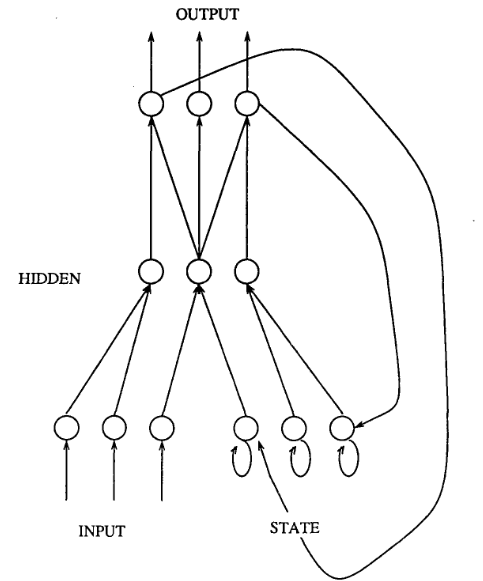
\includegraphics[width=.5\linewidth]{RNNIllustration.png}
        \caption[Schema of a Jordan Network]{Schema of a Jordan Network - \cite{elman1990finding}}
        \label{fig:RNNIllustration}
    \end{center}
\end{figure}

So, when evaluating a sample, the input layer receives not exclusively the values of the independent variables of the sample, but also some values that depend on the previous samples that were evaluated.
The ability to modify the output depending on the previous sample evaluated is what allows it to have some type of memory.
As discussed previously, this is an aspect very desirable for our problem.

Indeed, Xu \textit{et al.} \cite{Xu16} made use of recurrent neural networks to tackle the hard drive failure prediction problem.
Their setup for the neural network is quite standard, up until the point in which they introduce the concept of health status.

So, differently from every other approach in the literature they do not divide the samples in only two classes.
They actually use a more general method in which samples are divided in $N$ classes.

The ones from hard drives that do not fail during the observation period are given the label $N-1$.
The samples from failing disks are divided in the other $N-1$ classes, labeled from $0$ to $N-2$.
The algorithm they use to assign the failing samples divides them depending on how close they are to the failure by using fixed-length intervals.

We can formally define the approach that they explained in natural language in their paper as follows:
suppose that the last $n$ samples from each failing disk are kept in the training set and need to be divided in $N-1$ bins numbered from 0 to $N-2$.
Let the last sample from a specific hard drive before it fails be taken at time $T_i$.
Then, supposing that a sample is taken every 1 unit of time (usually once per hour) the class $c_i(t)$ of the sample of the disk $i$ at time $t$ is given by:

\begin{equation}\label{eq:linear_discrete_health_status}
  c_i(t) = 
  \begin{cases}
    & N-1 \text{, if } i \in \mathbf{healthy} \\
    & \biggl\lfloor(T_i-t)\dfrac{(N-1)}{n}\biggr\rfloor, 0 \leq T_i - t < n \text{, if } i \in \mathbf{failing}
  \end{cases}
\end{equation}

Here, $\lfloor x \rfloor$ is the floor of $x$, meaning the largest integer smaller than or equal to $x$.
For example, $\lfloor 1.8 \rfloor = 1$, $\lfloor 3 \rfloor = 3$.

By analyzing this formula, we see that the $\dfrac{n}{N}$ samples closest to the moment of failure are assigned to class 0, the next $\dfrac{n}{N}$ are assigned to class 1 and so on.

We can also prove that the formula indeed does what is desired, that is, it assigns a number from 0 to $N-2$ to each sample.
In order to do so, we notice that since we have $n$ samples, and the last one is taken at time $T_i$, the first one is taken at $T_i - n + 1$.

We can compute $c_i(T_i) = 0$ and $c_i(T_i - n + 1) = \biggl\lfloor(N-1)\left(1-\dfrac{1}{n}\right)\biggr\rfloor + 1$.
Since $\left(1-\dfrac{1}{n}\right) < 1$, $\biggl\lfloor(N-1)\left(1-\dfrac{1}{n}\right)\biggr\rfloor < N - 2$, so $c_i(T_i - n + 1) \leq N - 2$.
Moreover, $c_i(t)$ is clearly monotonic, since it is a composition of the floor function and elementary mathematical operations.

So, we can guarantee that the formula given above for $c_i(t)$ correctly assigns each sample to a class from $0$ to $N-2$ in which the closer the sample is to the moment the drive fails, the smaller is the value of its class label.

Here it is important to stress that even though both Xu \textit{et al.} \cite{Xu16} and Li \textit{et al.} \cite{Li14} use the term health status, they do not mean exactly the same thing.
The main distinction is that the latter used continuous values in order to train a regression tree, so, there is the idea of a class being closer or far apart from another.

The former, on the other hand, divides the samples in discrete, independent classes.

So, when training the recurrent neural network model, the $N$ classes are completely independent.
Concretely, it does not use the fact that when the correct output for a certain sample is 0, it is better to classify it as belonging to class 1 than to class $N-1$.

Even though the health status is a useful abstraction, there is a need to classify the sequence in itself in only two classes.

In order to do that, when they want to predict the status of a certain drive, they take its last $n$ samples.
Then, from the oldest to the most recent they put each sample as input to the network.
The order in which they are evaluated is important, since the model being used is an RNN and therefore has memory.

For each sample, they classify it as belonging to the class whose associated output neuron value is maximum.
By doing this, it is obtained a sequence of integers $c = (c_1, \dots, c_n), 0 \leq c_i \leq N-1$.

For each $j \in \{0,\dots,N-1\}$, let $C_j$ be the cardinality of $j$ in $c$.
It is clear that $\sum_{j=1}^N C_i = n$.
Then, they define two algorithms, the Voting Algorithm which Tends to Health (VAT2H) and the Voting Algorithm which Tends to Failure (VAT2F):

\begin{equation}\label{eq:vat2h}
    \text{VAT2H}(C) = 
    \begin{cases}
        & \text{Healthy, if } \sum_{j=0}^{N-3}C_j \leq C_N \\
        & \text{Failure, otherwise}
    \end{cases}
\end{equation}

\begin{equation}\label{eq:vat2f}
    \text{VAT2F}(C) = 
    \begin{cases}
        & \text{Healthy, if } \sum_{j=0}^{N-3}C_j < C_N \\
        & \text{Failure, otherwise}
    \end{cases}
\end{equation}

Notice that the contribution of the class $N-2$ is ignored in both algorithms.
This implies that these algorithms only work for when $N \geq 3$.

So, their approach is to extend the problem by expanding the number of classes from 2 to $N$ using equation \ref{eq:linear_discrete_health_status}.
Then, after the network classifies a sequence of samples of the same disk in the classes from 0 to $N-1$ they use equation \ref{eq:vat2h} or \ref{eq:vat2f} to obtain the final binary classification output.

They perform their tests on three different datasets corresponding to different models of hard drives.
The neural network for each model is trained independently since, as discussed, not only the behavior of hard drives of different models can be different \cite{Xu16}.

They obtained promising results with their method.
The FDR of their models was around 97\% while the FAR was almost always kept below 0.1\%.
As was expected, the VAT2H algorithm resulted in a lower FDR and a lower FAR than the VAT2F algorithm.

Nevertheless, their study admitted to having some limitation such as not studying the impact of other health status algorithms different from the one in equation \ref{eq:linear_discrete_health_status}.
Moreover, they used a fixed amount of classes with $N=6$ all over their research.

\section{Long Short-Term Memory}\label{sec:lstm}

Time has proved that RNNs are an effective method to tackle multiple sequence-based problems such as NLP \cite{tarwani2017survey} and video processing \cite{yadav2022survey}.

However, RNNs suffer from a limitation called the vanishing gradient problem.
This limits their efficiency when they need to learn long term dependencies.

This has been proven theoretically by Hochreiter \cite{hochreiter1998vanishing} as well as by Bengio \cite{bengio1993problem} using different approaches.
The intuition behind this result can be explained using the concept of error signal defined in Equation \ref{eq:error_signal}.

If we expand the bottom expression to explicitly write $e_i^{(l)}$ in terms of the error signals of layer $l+2$ instead of $l+1$, we obtain:

\begin{equation}
    e_i^{(l)} = \varphi '(u_i^{(l)}) \sum_j w_{ij}^{(l)} \left(\varphi '(u_j^{(l+1)}) \sum_k w_{jk}^{(l+1)} e_k^{(l+2)}\right)
\end{equation}

From this, we can see that $\dfrac{e_i^{(l)}}{e_i^{(l+2)}} \propto \varphi '(u_i^{(l)})\varphi '(u_j^{l+1})$.
So, it is proportional to the product of two derivatives.
We can extend this process to show that the impact induced by layer $l + m$ on layer $l$ must be scaled by the product of $m$ derivatives.

\begin{figure}
    \begin{center}
        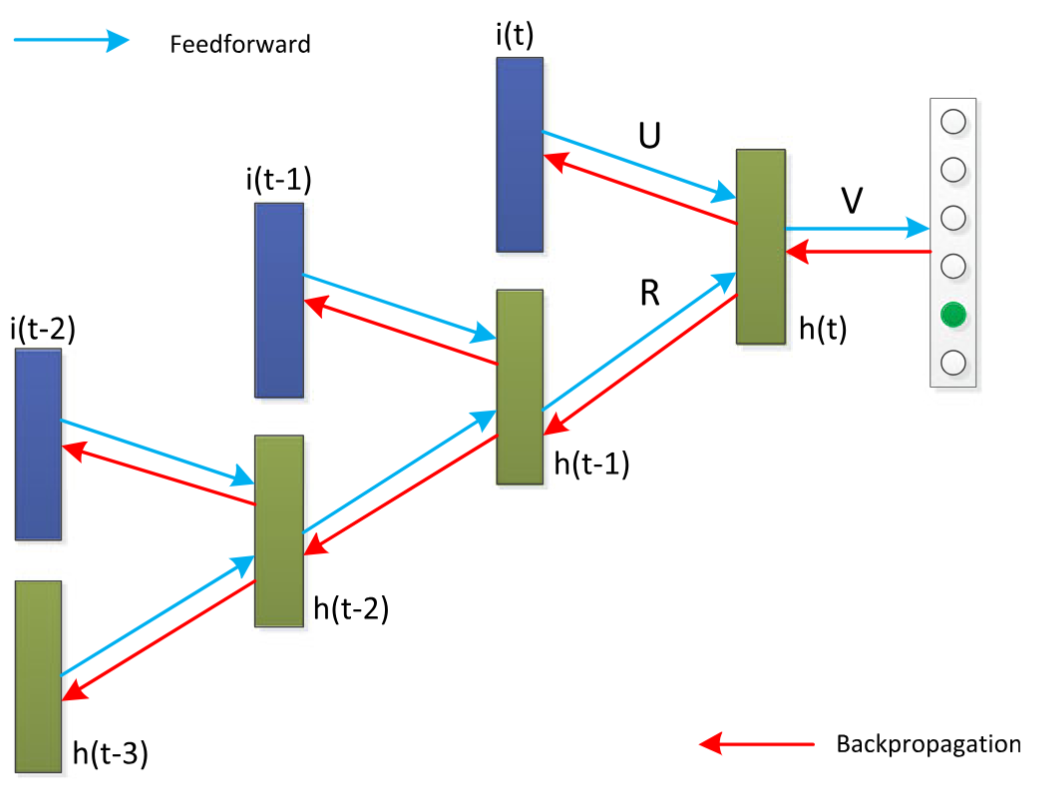
\includegraphics[width=.5\linewidth]{BPTT.png}
        \caption[Backpropagation Through Time]{Backpropagation Through Time interpretation of an RNN - \cite{Xu16}}
        \label{fig:BPTT}
    \end{center}
\end{figure}

But, if we redraw our RNN to be represented as in Figure \ref{fig:BPTT}, we see that the input of sample $t$ can be interpreted as being connected to the output of sample $t'$ by $(t'-t + 1)k$ layers, since it has to traverse the network with $k$ layers $t'-t+1$ times.
So the impact of the sample $t$ on sample $t'$ is proportional to $\prod_{i=1}^{(t'-t)k}\varphi'(x_i)$.

But, if the values of $\varphi'(x_i)$ are all smaller than 1, not only the scaling term will approach 0, but it will do so exponentially fast with respect to the distance between the two samples.

What Bengio showed on his paper \cite{bengio1993problem} is that, as a network learns, these derivatives decrease and become smaller than 1.
From this result, he was able to prove that, as the distance between two samples increase, the impact of the earlier one on the other on the RNN tends to zero.

The only assumption he made was that the model was not sensitive to noisy perturbations.
This is equivalent to stating that if two data sets are similar, then the model is able to learn approximately the same pattern, which is the case of every useful RNN.

So, there is a theoretical demonstration that for long enough sequences, the RNN architecture will be subject to the vanishing gradient problem.
However, theory alone is not enough to define what is a long enough sequence.
In order to state that the vanishing gradient problem has an impact on RNNs it is needed to observe such phenomenon in real-world scenarios. 

And, indeed, experiments show that problems as diverse as sentiment analysis \cite{raza2021cloud} and greenhouse gas predictions \cite{ludwig2019comparison} can be better learned by networks that try to solve the vanishing gradient problem such as LSTMs.

Other research projects show that applying techniques explicitly developed to curb the vanishing gradient problem can result in better results even without needing to change the architecture at all.
For instance, in \cite{hu2021handling} they adapted the activation functions by increasing the value of their derivatives and observed an improvement on the performance of the model.

With this evidence, both theoretical and experimental, it is clear the need to develop networks that are able to better handle or completely avoid the vanishing gradient problem.

So, after proving the vanishing gradient problem in RNNs, Hochreiter developed a network that did not suffer from this problem \cite{hochreiter1997long}.
His solution was the Long Short-Term Memory architecture.
A schematic view of such network is presented on Figure \ref{fig:LSTMSchema}.

\begin{figure}
    \begin{center}
        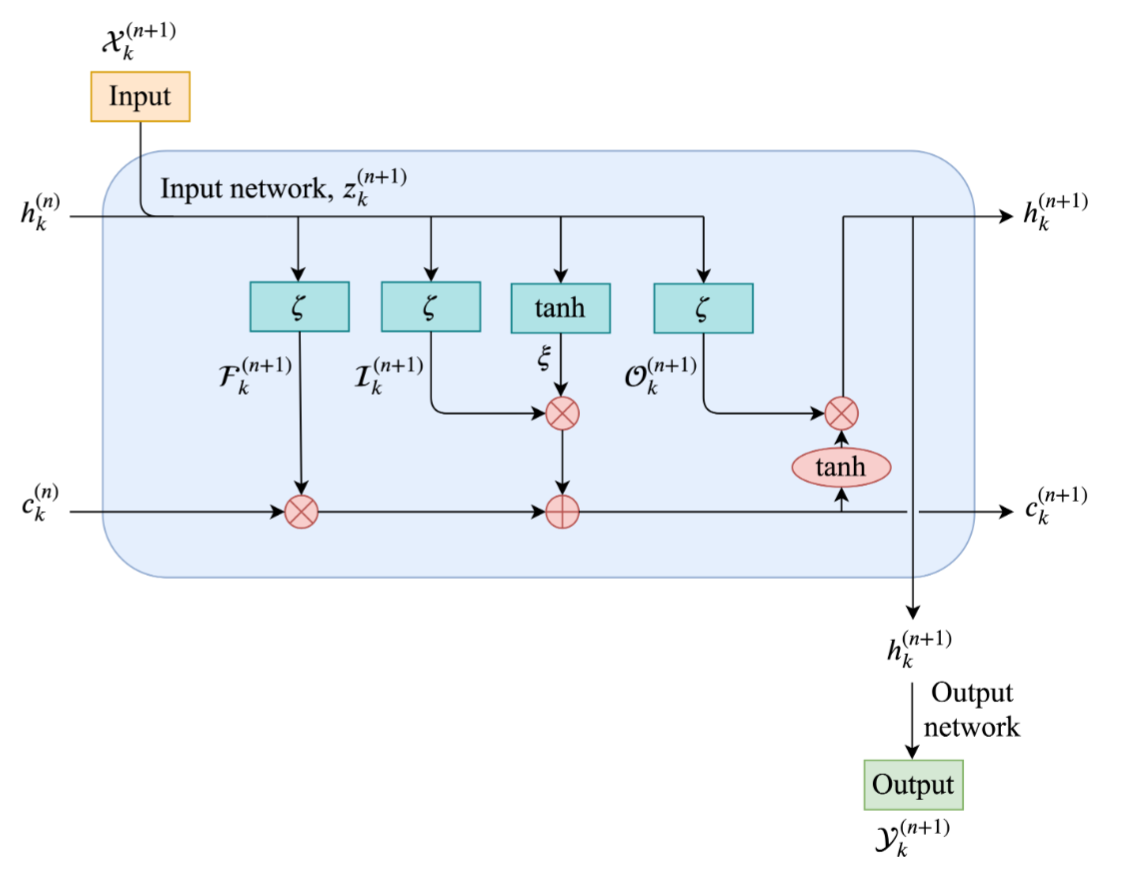
\includegraphics[width=.6\linewidth]{LSTM-Schema.png}
        \caption[Schema of an LSTM]{Schema of an LSTM - \cite{rahman2019nonintrusive}}
        \label{fig:LSTMSchema}
    \end{center}
\end{figure}

Similarly to the RNN architecture, we combine the output of the previous sample (represented by $h^{(n)}$ on the image) with the input data for the current sample ($\chi^{(n+1)}$).
However, the main innovation is the presence of the cell state: the channel represented by the horizontal lane in the bottom half of the image and dented by $c^{(n)}$.

It is not updated using the same logic of the neurons used by BPNNs and RNNs, so it is not subject to the vanishing gradient problem.
The operations performed by an LSTM can be explained in three steps, each one called a gate.

The first one is called the forget-gate and is represented in the image by the leftmost $\zeta$ node.
It takes the input of the current sample ($\chi^{(n+1)}$) and the last output ($h^{(n)}$) of the network and generates a forget-factor vector $P^{(n+1)}$ which is then multiplied component by component with the current value of the state $c^{(n)}$.

The name from this gate comes from the fact that it controls how much the network remembers from the past samples.
In the limit case in which $P^{(n+1)} = \mathbf{0}$, the value of $c$ is reset, and no information is kept from previous iterations.

The next step is the input gate, which in the image corresponds to the central $\zeta$ and $\tanh$ nodes.
If the forget gate decides how much from previous iterations should be kept in the cell state, the input gate controls which data from the current one should be added to the cell state.

The input gate is divided in two steps: the first is to generate the candidate values $\xi$ and the second is to compute the weights $I^{(n+1)}$.
Then each component of the candidate values vector is multiplied by its corresponding weight and added to the cell state.

Finally, there is the output gate that will actually compute the predicted output value for the sample.
In the image it is represented by the rightmost $\zeta$ and $\tanh$ gates.

This is the step that uses the cell state as input.
It combines the cell state value as well as the sample input $\chi^{(n+1)}$ and the previous sample output $h^{(n)}$ to compute a prediction $h^{(n+1)}$ for the current sample. 

In the previous paragraphs, we used generic terms such as compute and generate.
However, for an LSTM, the equations to calculate each term presented above is well-defined and are given by:

\begin{equation}\label{eq:lstm_calculations}
    \begin{cases}
        P^{(n+1)} &= \zeta(W_f\cdot[h^{(n)}, x^{(n+1)}] + b_f) \\
        I^{(n+1)} &= \zeta(W_i\cdot[h^{(n)}, x^{(n+1)}] + b_i) \\
        \xi &= \tanh(W_\xi\cdot[h^{(n)}, x^{(n+1)}] + b_\xi) \\
        C^{(n+1)} &= P^{(n+1)} \odot C^{(n)} + \xi \odot I^{(n+1)} \\
        O^{(n+1)} &= \zeta(W_o\cdot[h^{(n)}, x^{(n+1)}] + b_o) \\
        h^{(n+1)} &= O^{(n+1)} \odot \tanh(C^{n+1})
    \end{cases}
\end{equation}

In the equation above, $[x, y]$ is the concatenation of vectors $x$ and $y$ and $x \odot y$ is the Hadamard or element-wise product.
Also, $W_x$ and $b_x$ represent, respectively, the weights and bias of the network when computing variable $x$.
These are the values that need to be learned during the training process.

When it comes to applying this architecture to solving the hard drive failure prediction problem, there is not much relevant research about using LSTMs that has been published.
Nevertheless, there are some related works.

The first of them was done by Zhang \textit{et al.} \cite{zhang2017deep}.
The main objective of their work was to develop a symbolization-based feature extraction algorithm to improve event detection in LSTMs.

To show the impact of their approach they did perform an experiment on hardware failure detection.
However, they were presenting a more general method.
Consequently, they used different metrics such as balanced accuracy instead of FAR and FDR that would allow us to directly compare with other methods.

Despite us not having access do the desired metrics we can deduce some aspects of their results that allow us to compare to other works.
In order to do that, let positive be the event of the hard drive failing and negative the event of it not failing.

We then introduce the definition of Balanced Accuracy(BA), which was the metric used in \cite{zhang2017deep}:

\begin{equation}\label{eq:ba_def}
    BA \equiv \dfrac{1}{2}\left(\dfrac{TP}{TP + FN} + \dfrac{TN}{TN + FP}\right)
\end{equation}

But this is the average of the recall and the true rate negative, so we can plug the values from Equation \ref{eq:fdr_far} into Equation \ref{eq:ba_def} to obtain:

\begin{equation}
    BA = \dfrac{FDR + (1-FAR)}{2}
\end{equation}

So, even though it is not possible to retrieve the FDR and the FAR by themselves, it is possible to find a range of possible values for them from the balanced accuracy value.

In \cite{zhang2017deep}, the best BA they achieved over all the experiments with the LSTMs, with or without their feature extraction algorithm, was $85.2\%$.
But, since BA is the average of FDR and $(1-FAR)$, it implies that one of these values is at most $85.2\%$, else their average would be bigger.

So, either the FDR they achieved is under $85.2\%$ or their FAR is above $14.8\%$ which is much worse than the one achieved with any other methods we have discussed.

This indicates that their research cannot be used as a reference for the Hard Disk Failure Detection Problem.

There is an additional paper by Das \textit{et al.} \cite{das2018desh} that also applies LSTM to hardware failure detection.
However, it is not for hard drives in data centers, but rather to nodes in a supercomputer which leads to a profile much different from the papers discussed so far.

The first notable difference is that the time scales in which it operates is much smaller.
The TIA they achieve is of the order of 100 seconds, which shows a behavior unlike the one found in data centers in which it is possible to predict a failure more than 100 hours in advance \cite{Li14} \cite{Zhu13}.

But the most important difference is that in \cite{das2018desh} they try to predict failures that happen in components other than the hard drive.
So, they do not make use of SMART attributes, they instead analyze system logs.

Therefore, their motivation to use LSTMs is to detect patterns in text rather than to study time-series.

The FDR they achieve with their LSTM-based approach is between $85.1\%$ and $87.5\%$.
However, it is not possible to compare it to the other results presented above since their problem is quite different from the detection of hard drive failures in data centers.

\section{Additional State of the Art methods}

There are a few additional methods that have been used to tackle the hard drive failure prediction problem and that are worth mentioning.
Since these approaches will not be implemented by our current work, we will limit ourselves to a briefer explanation of the theory behind them.

\subsection{Random Forest}\label{subsec:randomforest}

One of the problems faced by decision trees, specially when they become large is overfitting \cite{ying2019overview}.
This is due to the fact that the split values for each attribute used by the tree are directly taken from the values on the training set.
So, when the tree is deep and there are only a few training samples in a node, the splitting values will sharply follow the ones in the training set.
This is what leads to overfitting \cite{Bramer2020}.

In order to tackle this, Random Forests has been introduced \cite{ho1995random}.
The idea is to train multiple, independent decision trees at once, each one trained with a different subset of the training data.
Notice that these subsets do not have to be disjoint, specially when the training set is relatively small.
This approach reduces the probability of overfitting, since a sample will not be seen by some trees.

Random Forests have performed well for a variety of tasks, ranging from image recognition to Alzheimer's disease detection and prediction \cite{shaik2019brief}.

Research by Shen \textit{et al.} \cite{Shen18} used Random Forests for hard drive failure prediction.
One of the most interesting aspects of their research is how they combined the results of the different trees of the forest in order to evaluate a sample.

Their approach is to not simply feed a sample to every tree in the forest and check which of the two outputs appeared more frequently.
Instead, they gave different weights to the output of each tree based on a clustering algorithm.

More specifically, they performed two independent clustering processes, one for the failing and another to the non-failing samples.
Then, when predicting the outcome for an unseen sample, the clusters $c_0$ and $c_1$ to which it would belong if it were failing or non-failing sample, respectively, are computed.

Since it is known which samples of the training set were used to train each tree, it is possible to evaluate the accuracy of each tree for the training samples in $c_0$ and in $c_1$.
Based on these accuracies, it is possible to give a bigger weight to trees that better learned the samples of the clusters to which the sample being evaluated belongs.

They used a simple algorithm in which the weight of a tree is either $0$ or $1$.
If a tree output a prediction that the current sample being evaluated corresponds to a failing disk, its vote will only be taken into account if its accuracy for samples in $c_0$ that also belong to the training set of the tree is at least $0.5$.
The same will be doing if the prediction of the tree is of a healthy disk, but instead its accuracy will be evaluated over the disks in $c_1$.

Despite this simplicity, they were able to achieve a great performance.
The FDR obtained was above 98\% while the FDR was kept under 0.1\% for multiple scenarios.

What allowed them to get these excellent outcomes, besides of course the algorithm, was their dataset that contained more than 2 million samples of SMART attribute snapshots.

\subsection{Support Vector Machine}

A Support-Vector Machine (SVM) is a non-probabilistic classifier \cite{cortes1995support}.
The idea behind it is to plot the samples in an $n$-dimensional space, in which $n$ corresponds to the number of features in the vector.

Then, the algorithm finds the hyperplane that minimizes its loss function.
The points on one side of the hyperplane correspond to the positive class and the other to the negative class.

The main drawback of SVMs is that drawing a hyperplane means that it can only detect linear dependencies.
So, if there are points in a 2D-plane and the boundaries between the healthy and failing classes is the circumference centered at the origin with radius 1, there is no way that a line can be drawn to correctly divide both regions.

The solution to this is to use the kernel-method, in which dimensions of the original vector are combined using non-linear function and the output of the function is assigned to a new component of the sample vector.
This allows the SVM to correctly learn non-linear dependencies between the variables.

Suppose we want to identify two classes of points that are described by points in a plane.
A class is denoted by the points inside the circle centered at the origin with radius one and the other are all other points.
It is impossible to draw a line in two dimensions that correctly separates both classes.

However, in this example, we can transform the vector $v = (x, y)$ into $v' = (x, y, x^2 + y^2)$ and then and apply the SVM to the set of $v'$.
Then the SVM can potentially learn the plane $z = 1$ (or something similar to it) and thus solve the classification problem without needing to learn explicitly non-linear dependencies.

When it comes to applying SVMs to predicting hard drive failure, the best results were achieved in \cite{Zhu13}.
They used hyperparameters on their model in order to prioritize either a small FAR or a big FDR.

When optimizing for the smallest FAR possible, Zhu \textit{et al.} obtained a FAR of $0.03\%$ and an FDR of $68.5\%$.
When priority was giving to increasing the FDR, they obtained a FAR of $0.3\%$, but the FDR was increased to $80.0\%$.

Support-Vector Machines, when compared to other approaches, present, therefore, a method that is able to achieve a smaller FAR.
However, in contrast, it is not able to attain FDRs as good as other methods while keeping an acceptable FAR.

\subsection{Linear Regression}

An approach using one of the simplest statistical learning methods, linear regression, has been proposed for the hard drive failure prediction problem.
Yang \textit{et al.} \cite{yang2015hard} showed described a methodology to obtain good results with a linear regression model.

In order to allow a simple method to detect rather complex relationships as the ones that can occur between the value of SMART attributes, the focus of their work was on feature engineering.
More specifically, they started by dividing values of each SMART attribute in different bins.
Then, depending on the bins occupied by the attributes of a hard drive, the SMART values were translated in a set of features.

Since some specific combinations of bins were required for the algorithm to assign a certain feature to a hard drive, the feature space was sparse.
This means that a single disk did not satisfy the conditions to be assigned most of the features.

The main drawback of this approach is the need for massive amounts of data.
In their work they state that their dataset, consisting of more than 7 million samples, contains 500 times more samples of SMART attributes than any other work on this problem.
Not only this data may be not trivial to obtain, but also it is accompanied by a necessity of a substantial computing infrastructure to process it.

An important aspect of their approach is that no distinction was made between hard drives whose models were different.
This is a sharp contrast with other research on the subject that explicitly train different machine learning models for different disk models \cite{Xu16} \cite{Shen18} \cite{Li14}. 

Despite this limitation, their results were promising, showing an FDR of 97.8\% with an FAR of 0.3\%.
However, they also showed that the huge amount of data they used to train their model is a non-negotiable requirement.
For a subset that only included 1/512 of the original dataset samples, meaning that its size was comparable to the one in other works, even for an FDR of 0.5\%, the FDR is below 40\%, which is much worse than other work done on the same problem.

\subsection{Convolutional Neural Networks}

A Convolutional Neural Network (CNN) is a machine learning model.
It is usually applied to computer vision tasks.
Just like BPNNs discussed in Section \ref{sec:BackpropagationNeuralNetwork}, it is not recurrent meaning that the output for a certain sample is not propagated to following ones.

The main aspect that differs a CNN from a BPNN is the presence of convolutional layers \cite{o2015introduction}.
In a convolutional layer, a neuron in layer $l$ is not connected to every neuron in layer $l-1$.
Instead, it is connected to a few consecutive nodes of layer $l-1$.

This is useful for handling data that is represented as a vector with many components, such as images, in which each pixel corresponds to an input.
For a 100x100 image, fully connecting two layers would require 10,000 weights.
By using a 5x5 convolution window with shared weights, it is possible to reduce this value to only 25 weights, or 400 times less.
This allows the network to be much deeper.
 
A relevant attribute of a CNN is its translation invariance \cite{kayhan2020translation}.
The use of shared weights implies that shifting some values by a certain constant value does not hinder the network's ability to recognize a certain pattern.
This is because the convolutions will be performed with the same weights no matter in which part of the image a certain sequence of values is.

It was exactly this translation invariance aspect of the CNN that motivated Sun \textit{et al.} \cite{sun2019system} to adapt CNNs to handle time series to tackle the hard drive failure prediction problem.
For a time-series, translation invariance implies that a pattern due to a sequence of values or events can be detected independently of where in the sequence it occurs.

In order to obtain, they also had to adapt the loss function to handle the imbalanced dataset that contained many more healthy samples than failing ones, which is an intrinsic aspect of the problem at hand.

So, they gave a bigger weight to samples from failing disks that were misclassified, else the model would be prone to classify almost every disk as a healthy one.
This is due to the fact that, with a classic loss function, even if the model misclassified every failing disk, its total loss would be much smaller than if it misclassified even a small percentage of the healthy disks.

In their results, the metric they presented that we can use to compare with other methods was the recall, which corresponds to the FDR.
They achieved an FDR of $65\%$ which is considerably smaller than the one attained by other models.
But this is partly due to the fact that they used a heterogeneous dataset, meaning that they did not train different networks for different hard drive models.